\documentclass[11pt, a4paper]{article}

\usepackage{graphicx}
\usepackage[a4paper,top=3cm,bottom=2cm,left=2cm,right=2cm,marginparwidth=1.75cm]{geometry}
\usepackage[english]{babel}
\usepackage[utf8x]{inputenc}
\usepackage{subfig}
\usepackage{float}
\usepackage{amsmath}
\usepackage{amssymb}
\usepackage{mhchem}
\usepackage{hyperref}
\usepackage{tikz}
\usepackage{cancel}
\usepackage{bm}

\graphicspath{ {./images} }
\newcommand*{\qed}{\hfill\ensuremath{\quad\square}}%
\newcommand*{\rad}{\ensuremath{\,\text{rad}}}
\newcommand*{\R}{\ensuremath{\mathbb{R}}}
\newcommand*{\C}{\ensuremath{\mathbb{C}}}
\renewcommand*{\Re}{\operatorname{Re}}
\renewcommand*{\Im}{\operatorname{Im}}
\renewcommand*{\epsilon}{\varepsilon}
\renewcommand*{\phi}{\varphi}
\renewcommand*{\d}{\,\text{d}}

\DeclareRobustCommand{\uvec}[1]{{%
  \ifcat\relax\noexpand#1%
    % it should be a Greek letter
    \bm{\hat{#1}}%
  \else
    \ifcsname uvec#1\endcsname
      \csname uvec#1\endcsname
    \else
      \bm{\hat{\mathbf{#1}}}%
     \fi
   \fi
}}

\makeatletter
\renewcommand*\env@matrix[1][*\c@MaxMatrixCols c]{%
  \hskip -\arraycolsep
  \let\@ifnextchar\new@ifnextchar
  \array{#1}}
\makeatother

\newtheorem{theorem}{Theorem}
\numberwithin{equation}{section}
\numberwithin{figure}{section}

%------------------------------------------------
%Templates for images and figures
% \begin{figure}[h]
%   \centering
%   \subfloat[caption 1]{{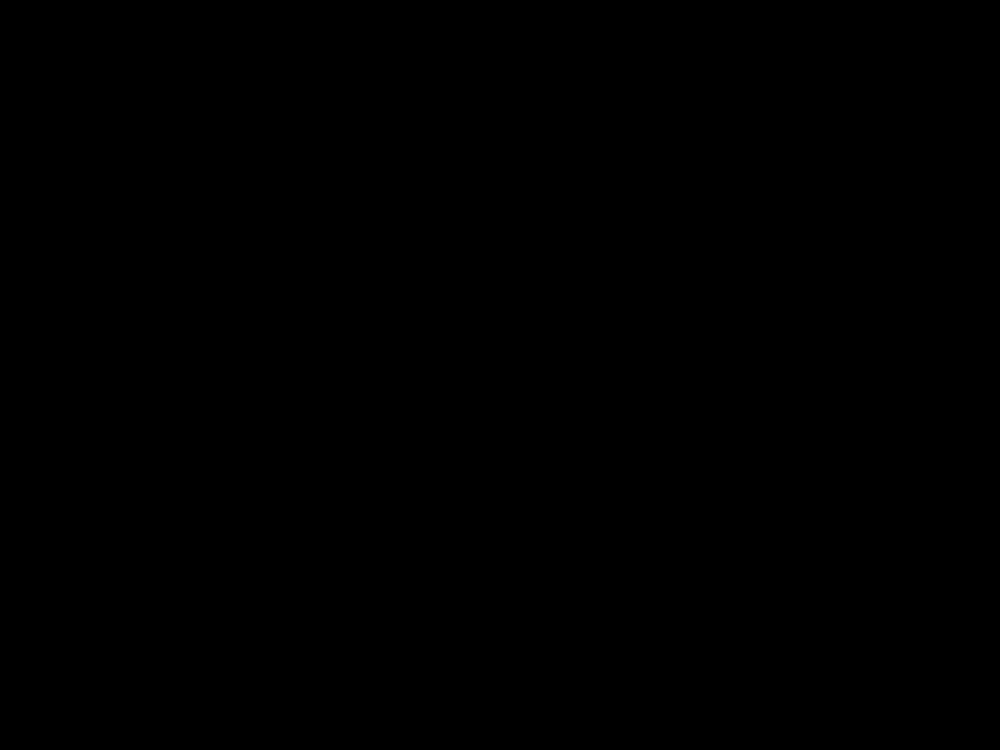
\includegraphics[width=30mm]{images/placeholder.png}}}%
%   \qquad
%   \subfloat[caption 2]{{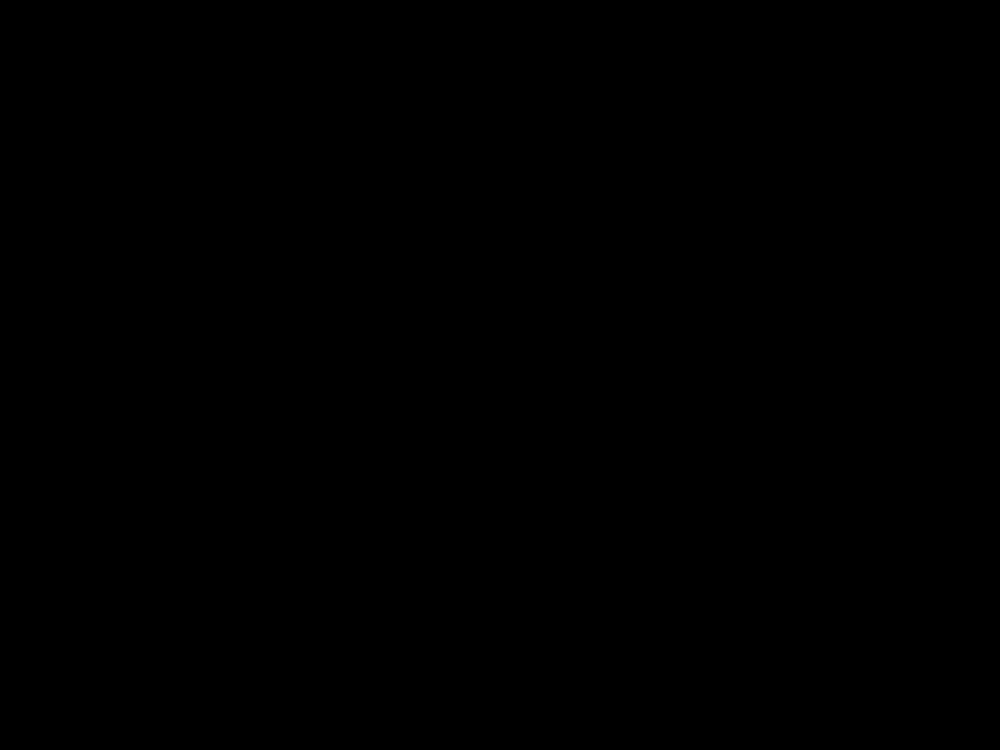
\includegraphics[width=30mm]{images/placeholder.png}}}%
%   \caption{Description}
% \end{figure}

% \begin{figure}[h]
%   \centerline{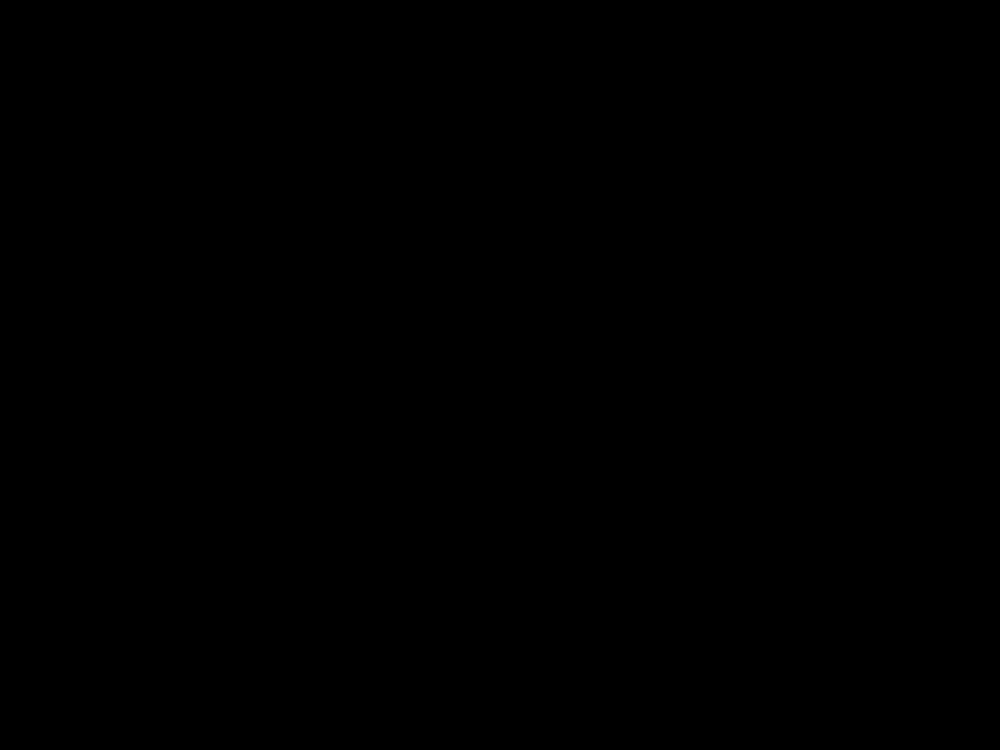
\includegraphics[width=50mm]{images/placeholder.png}}
%   \caption{Description}
% \end{figure}

%Template for a simple table 
%\begin{table}[h]
%   \caption{Description} %title of the table
%   \centering % centering table
%   \begin{tabular}{l rr} % creating three columns
%     \hline\hline %inserting double-line
%     & & \\ [0.5ex] % Insert half line vertical spacing
%     \hline % inserts single-line
%     & & \\ 
%     & & \\
%     & & \\
%     & & \\
%   \hline % inserts single-line
%   \end{tabular}
%   \label{tab:hresult}
% \end{table}
%-----------------------------------------------

\begin{document}
\setcounter{section}{2}

\section{The Cauchy stress tensor}
\subsection{Differential elements of force and the stress vector}
Consider the following situation where the plane $\d A$ is some differential material element oriented within the material. The vector $\uvec{n}$ is normal to this plane and thus encodes it's orientation in space. We know from mechanics of materials that the internal stress in per unit of area. This means we can find the localized stress using the force acting on the area element and the area:
\begin{equation}
  \vec{p} = \lim_{\Delta A \to 0} = \frac{\Delta \vec{F}}{\Delta A} \Rightarrow \d \vec{F} = \vec{p}\d A
\end{equation}
Where $\vec{p}$ is the localized stress of the differential material element $\d A$ encoded using the stress vector. Note that the resulting stress vector is dependent on the choice of the plane orientation as well as spatial position. This can be related back to Mohr's circle.
\begin{figure}[H]
  \centerline{\includegraphics[width=80mm]{images/stress_element.png}}
  \caption{Variation of the stress vector $\vec{p}$ with the normal vector $\uvec{n}$.}
\end{figure}
We can represent the stress vector using the normal vector of the plane $\uvec{n}$ and the stress tensor.
\begin{gather}
  \vec{p}(x, n) = \mathbf{\sigma}(x) \uvec{n}\\
  \begin{bmatrix}
    p_x \\
    p_y \\
    p_z
  \end{bmatrix}
  =
  \begin{bmatrix}
    \sigma_{xx} & \sigma_{xy} & \sigma_{xz} \\
    \sigma_{yx} & \sigma_{yy} & \sigma_{yz} \\
    \sigma_{zx} & \sigma_{zy} & \sigma_{zz} \\
  \end{bmatrix}
  \begin{bmatrix}
    n_x \\
    n_y \\
    n_z
  \end{bmatrix}
\end{gather}
\begin{figure}[H]
  \centering
  \subfloat[2D]{{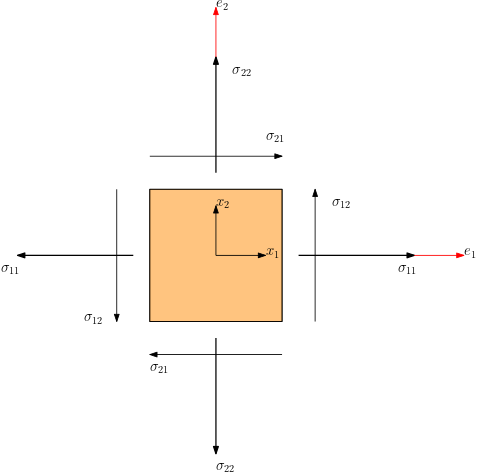
\includegraphics[width=60mm]{images/2D.png}}}%
  \qquad
  \subfloat[3D]{{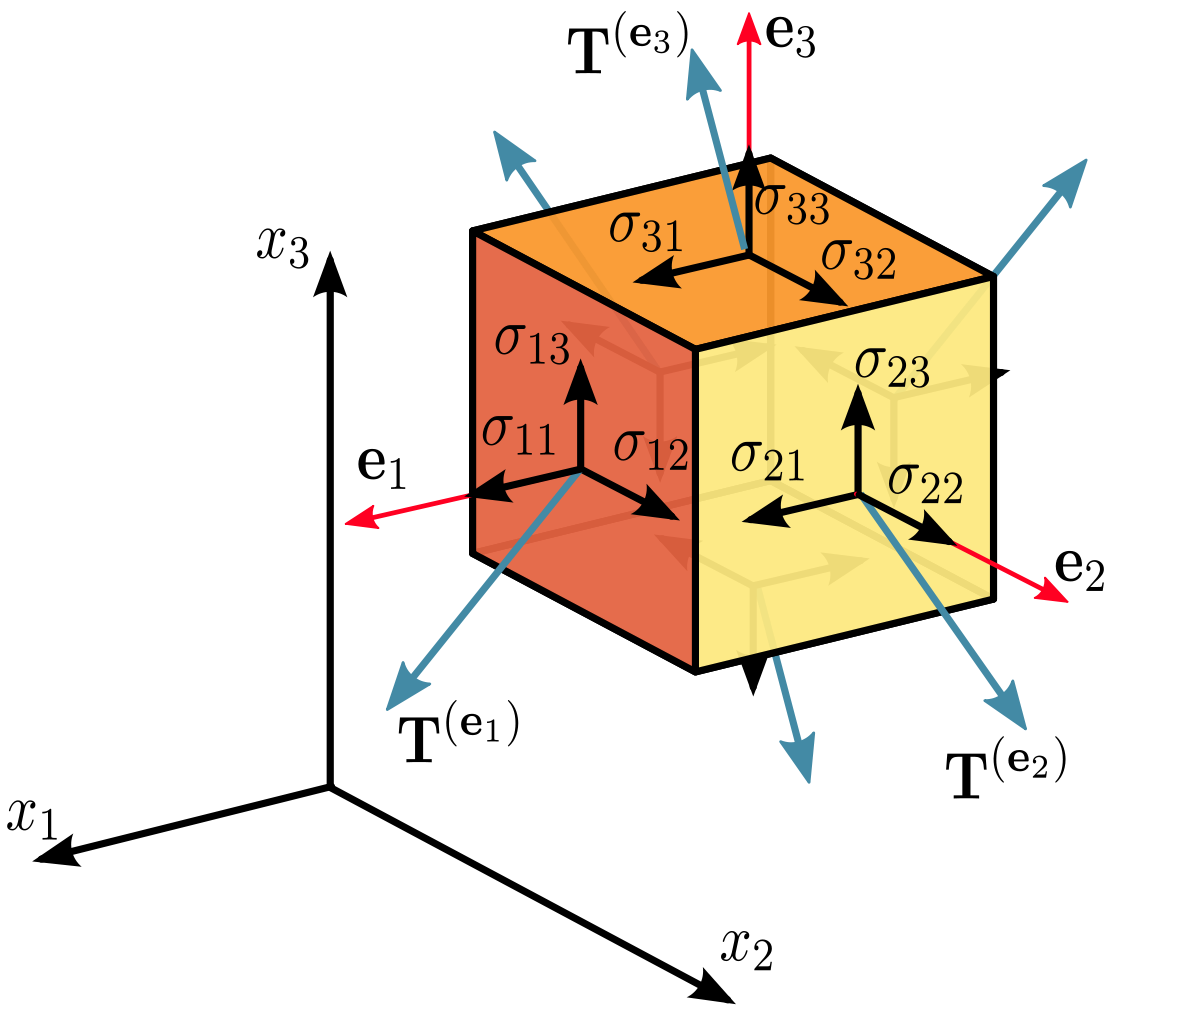
\includegraphics[width=60mm]{images/3D.png}}}%
  \caption{The components of the stress tensor acting on some material element represented in 2D and in 3D. Source: \url{https://en.wikipedia.org/wiki/File:Components_stress_tensor_cartesian.svg}}
\end{figure}
We can divide the components of the stress tensor into 2 main components: Shear stresses along the plane with normal $\uvec{n}$ and normal stresses which are normal to the plane and by extension parallel to $\uvec{n}$. The normal stress is a scalar quantity and can be found using:
\begin{align}
  \sigma_n &= \vec{p} \cdot \uvec{n} \notag\\
           &=
  \begin{bmatrix}
    n_x &
    n_y &
    n_z
  \end{bmatrix}
  \begin{bmatrix}
    \sigma_{xx} & \sigma_{xy} & \sigma_{xz} \\
    \sigma_{yx} & \sigma_{yy} & \sigma_{yz} \\
    \sigma_{zx} & \sigma_{zy} & \sigma_{zz} \\
  \end{bmatrix}
  \begin{bmatrix}
    n_x\\
    n_y\\
    n_z
  \end{bmatrix}
\end{align}
The shear stress is a vector quantity and is found using:
\begin{equation*}
  \vec{\sigma}_s = \vec{p} - \sigma_n \uvec{n}
\end{equation*}
The magnitude of the shear stress can be found by taking the norm of $\vec{\sigma_s}$. Dividing stress in these 2 components is usefull for quantifying shear stresses along layers of glue of other adhesion material for example.
\begin{figure}[h]
  \centerline{\includegraphics[width=40mm]{images/stress_vector.png}}
  \caption{The graphical interpretation of the stress components $\sigma_n$ and $\vec{\sigma}_s$}
\end{figure}

\subsection{Equilibrium conditions}
The stress tensor has to be symmetrical to statisfy the angular equilibrium condition. This means that:
\begin{equation}
  \sigma_{ij} = \sigma_{ji}
\end{equation}
To the statisfy the linear equilibrium conditions we find that:
\begin{equation}
  \sum_{j=1}^3 \frac{\partial \sigma_{ij}}{\partial x_j} + \rho f_i = 0 \quad \text{for} \quad \vec{x}\in V
\end{equation}
Where the term $\rho f_i$ represents loadings per unit mass of the material such as gravity acting on the material. We have 3 spatial coordinates so this can be written in terms of a system of 3 equations as:
\begin{equation}
  \begin{cases}
    \sigma_{xx,x} + \sigma_{xy,y} + \sigma_{xz,z} + \rho f_x = 0\\
    \sigma_{yx,x} + \sigma_{yy,y} + \sigma_{yz,z} + \rho f_y = 0\\
    \sigma_{zx,x} + \sigma_{zy,y} + \sigma_{zz,z} + \rho f_z = 0\\
  \end{cases}
\end{equation}
There is one final condition for equilibrium which states that:
\begin{equation}
  \sum_{j=1}^3 \sigma_{ij} n_j = q_i \quad \text{for} \quad \vec{x}\in A_p
\end{equation}
This means that when we consider the stress at the surface of the material denoted as the set of all points in $A_p$ the stress inside the stress from the material element we are considering must be in equilibrium with some externally applied load $\vec{q}$.

\subsection{Notation}
The stress tensor is sometimes also denoted as:
\begin{align}
  \mathbf{\sigma} &= 
  \begin{bmatrix}
  \sigma_{xx} &  \sigma_{yy} &  \sigma_{zz} &  \sigma_{xy} &  \sigma_{yz} &  \sigma_{zx}
  \end{bmatrix} \notag \\
  &=
  \begin{bmatrix}
    \sigma_{xx} &  \sigma_{yy} &  \sigma_{zz} &  \tau_{xy} &  \tau_{yz} &  \tau_{zx}
    \end{bmatrix}
\end{align}

\end{document}